% When draft option is activated, lines are numbered.
\documentclass[draft]{trb_unofficial}
\usepackage{graphicx}

% Put here what will go to header as author
\AuthorsHeading{Pritchard, Macfarlane, and Wang}
\title{A \LaTeX\ Template for Papers Submitted to the Transportation
Research Board}

% TODO: add macros for easier formatting of \author.
\author{
  \textbf{David Pritchard} \\
  davidpritchard.org\\[12pt]
  \textbf{Gregory S. Macfarlane, Ph.D.}\\[12pt]
  \textbf{Chieh (Ross) Wang, Ph.D.}\\
  cw@crosswang.org
}

\begin{document}
\thispagestyle{empty}

\maketitle
\section{Abstract}
%% ***   Put your Abstract here.   ***
%% (At most 250 words.)

The Transportation Research Board has unique and seemingly arbitrary
requirements for manuscripts submitted for review. These requirements make it
difficult to write the manuscripts quickly, and no existing \LaTeX\ style comes
close to fooling the guidelines. This represents an initial effort at creating a
template to meet the requirements of TRB authors using \LaTeX, R, Sweave, and/or other
literate programming software.

\newpage

\section{Introduction}
The \trbcite{TRBGuide} has unique and somewhat arbitrary requirements
for papers submitted for review and publication. While the initial submission is
required to be in PDF format, submissions for publication in Transportation
Research Record must be in Microsoft Office format. On top of this, the
manuscripts must be line-numbered, captions are bolded and employ atypical
punctuation, and the references must be numbered when cited and then printed in
order.

It is assumed that the readers of this document have some significant level of
experience in \LaTeX and \verb1bibtex1. As use of literate programming becomes more
widespread in engineering and planning, it is possible that this template may
need to be made more robust.

\subsection{History}
David Pritchard posted the original versions of this template in 2009 and
updated it in 2011, soon after TRB began allowing PDF submissions. Gregory
Macfarlane made significant adaptations to it in March 2012, allowing for Sweave
integration and automatic word and table counts. Ross Wang automated the
total word count and made some formatting modifications in July 2015. Version 2.1.1 has been made available on GitHub in January, 2016.  Version 2.1.1 Lite was made available on GitHub in June, 2017.



\section{Features}
The template has a number of features that enable quick and painless manuscript
authoring.

\subsection{Title Page}
The standard \LaTeX\ \verb1\maketitle1 command is not very versatile, so we have
replaced it with a \verb1titlepage1 environment. This means that the writers
will be required to manually enter spacings based on the number of contributors,
but the current settings (12pt between authors, 36pt before, and 60pt after them)
seems to work well. 

Near the bottom of the title page, TRB requires a count of the manuscript's
words, figures, and tables. This template generates these counts automatically.
The figure and table counts are simply pulled from the \LaTeX\ counters using the
\verb1totcount1 package. The word count feature is not as straight-forward, as it
utilizes a call to the system command \verb1texcount1. Thus to compile the
document writers must enable \verb#\write18# in their \verb1pdflatex1 call.

In the newest version of this template, we added the total count automatically. 
The total count basically adds not only the word count, but also the equivalent
count (250 words) for each figure and table.  This is implemented using a cusomized
command \verb1\totalwordcount1.  Please see the original code for more information.

\subsection{Page Layout}
The document has 1 inch margins as required, with the author's names in the left
heading and the page number in the right. The authors heading will need to be
edited by the writers; automating this from the title page command is not
currently possible. Paragraphs leading sections and subsections are not
indented, while all subsequent paragraphs in that section are. Section types are
defined as outlined by the \trbcite{TRBGuide}

The document is single-spaced in 12 point Times font. Times New Roman is a
proprietary font and is therefore not available by installation in open-source
software. While the differences between Times variants are negligible, Times New
Roman itself can be used in Mac OSX by compiling under \verb1xelatex1.

\subsubsection{Line Numbers}
Manuscript line numbering is implemented using the \verb1lineno1 package. There
are options to change the font style and type, but the current settings work
well. Note that the line numbers refresh each page, and that blank lines do not
receive a number.  Currently, line numbers and headers are not shown on the title page, but can be easily added by adding \verb1\pagewiselinenumbers1 command right before the beginning of the title page.

\section{Captions}
Figure \ref{fig:trial} shows a Gumbel distribution as an example of captioning.
As demonstrated, figure captions ought to be sentence capitalized, bolded, and
can be somwhat longer than in other journals.

Table captions are somewhat different, requiring initial capitals and are more of a
title. An example of this is given in Table \ref{tab:versions}, showing the
history of this template.

\begin{figure}[t]
  \centering
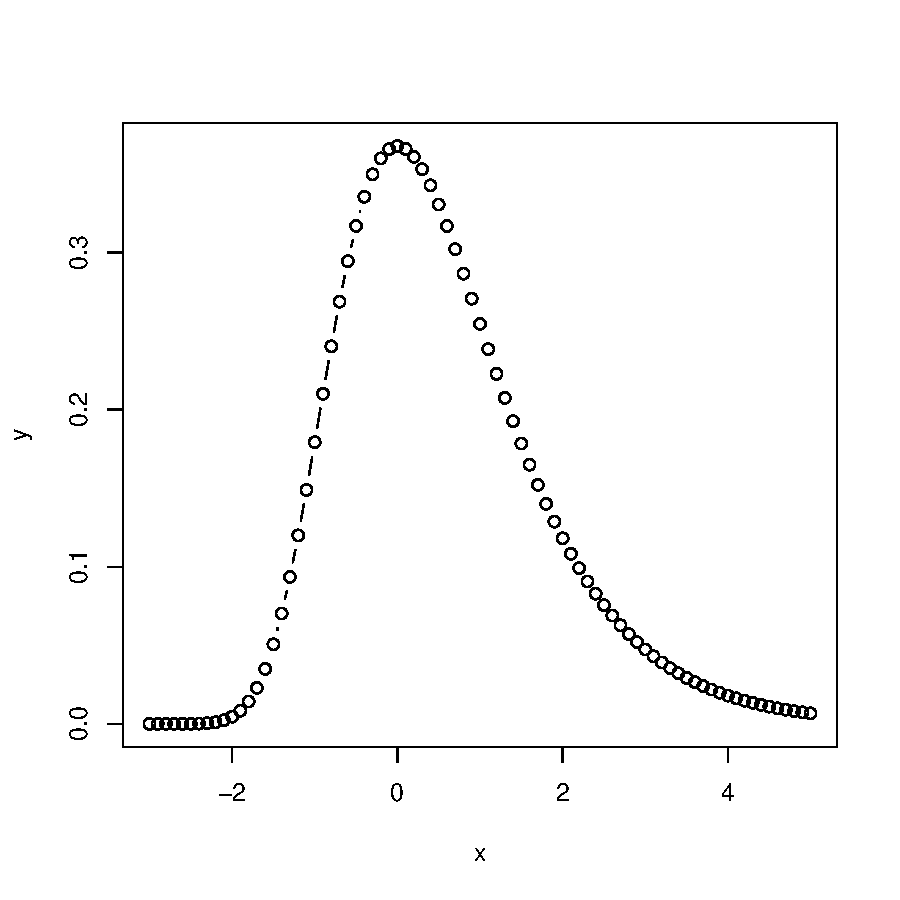
\includegraphics{trb_template-gumbel}
\caption{This is a random figure to test the counting functionality on the
title page. It shows a Gumbel distribution with mode 0 and scale 1. The
multinomial logit model assumes that the error terms are distributed identically
and independently following this pattern.}
	\label{fig:trial}
\end{figure}

\begin{table}[t]
  \caption{A History of this Template}
	\label{tab:versions}
\begin{center}
	\begin{tabular}{l l l l}
Version & Date & Author & Contributions \\\hline
1.0   & Sep 2009 & Pritchard & Initial work \\
1.1   & Mar 2011 & Pritchard & Captions \\
2.0   & Mar 2012 & Macfarlane& Automation, documentation\\
2.1   & Jul 2015 & Wang      & More automation and formatting\\
2.1.1 & Jan 2016 & Wang      & Minor modifications and uploaded to Github\\
2.1.1 Lite & Jun 2017 & Wang & TeX-only template \\\hline
\end{tabular}
\end{center}
\end{table}

\subsection{Bibliography}
The TRB bibliography style is defined in the \verb1trb.bst1 file which should be
in your document folder. A new command is specified, \verb1\trbcite{}1 which
will print the authors and the number of the reference in the order in which it
is supplied. Note that \verb1\trbcite{}1 prints both the author names and the reference number, if you simply need the number of the reference, use command \verb|\cite{}|. The References section will be appended to the end of the document.

It is very easy to add reference to papers programs written by
\trbcite{Bierlaire2003} and \trbcite{Bierlaire2008} or to papers like those
written by \trbcite{Garrow2009} and \trbcite{Koppelman2005}. You can even go
back and refer to Biog\'eme by \trbcite{Bierlaire2008} a second time.  You can also cite a group of similar references without printing author names \cite{TRBGuide,Bierlaire2003}.  This template also groups multiple reference numbers together if there are three or more consecutive numbers \cite{Bierlaire2003,Bierlaire2008,Garrow2009,Koppelman2005}.

\section{To Do's}
There is still work to be done on this template. Currently, the word count
feature includes text in the abstract. 

There may be other important features in the template that we have not
considered. Ideally, we would make a \verb1trb.sty1 style class that could be
called and we would not have to expose the user to so much \TeX-ese. This could
be forthcoming, but not for this TRB cycle. 

\section{Conclusion}
To make the document from source in a Unix-like OS using Sweave, issue the following
commands:
\begin{verbatim}
R CMD SWEAVE 'trb_template.rnw'
pdflatex --shell-escape document.tex
bibtex document
pdflatex --shell-escape document.tex
pdflatex --shell-escape document.tex
\end{verbatim}
The \verb1--shell-escape1 option is required to access the command line for the word count. Normally this feature is disabled because it is a route of entry for malicious software. We promise that there is no such debilitating code in this document, and we encourage you to examine any scripts for suspicious code before permitting \verb1pdflatex1 from accessing your system.

For R-Studio users using Sweave and .rnw files, you may enable shell escape command in the Global Options > Sweave settings.  Moreover, if your computer does not have a Perl interpreter you will need one, such as the ActivePerl, for the wordcount to work properly.

\newpage

\bibliographystyle{trb}
\bibliography{trb_template}

% End line numbering
\nolinenumbers
\end{document}
